\chapter{Lec TBL - Classification}

\section{Classification}
The linear regression model discussed before assumes that the response variable $Y$ is quantitative. But in many situations, the response variable is instead qualitative. For example, eye color is qualitative, taking on values blue, brown, or green. Often qualitative variables are referred to as categorical; we will use these terms interchangeably. In this chapter, we study approaches for predicting qualitative responses, a process that is known as classification.\\\\
Classification problems occur often, perhaps even more so than regression
problems. Some examples include:
\begin{itemize}
    \item A person arrives at the emergency room with a set of symptoms
    that could possibly be attributed to one of three medical conditions.
    Which of the three conditions does the individual have?

    \item An online banking service must be able to determine whether or not
    a transaction being performed on the site is fraudulent, on the basis
    of the user’s IP address, past transaction history, and so forth.

    \item On the basis of DNA sequence data for a number of patients with
    and without a given disease, a biologist would like to figure out which
    DNA mutations are deleterious (disease-causing) and which are not.
    
\end{itemize}
Just as in the regression setting, in the classification setting we have a
set of training observations $(x_1, y_1),...,(x_n, y_n)$ that we can use to build
a classifier. We want our classifier to perform well not only on the training
data, but also on test observations that were not used to train the classifier.

\section{Why Not Linear Regression?}
\label{lin_reg}
We have stated that linear regression is not appropriate in the case of a
qualitative response. Why not? Suppose that we are trying to predict the medical condition of a patient in the emergency room on the basis of her symptoms. In this simplified example, there are three possible diagnoses: \textit{stroke}, \textit{drug overdose}, and \textit{epileptic seizure}. We could consider encoding these values as a quantitative response variable, $Y$, as follows:
\[
Y = \begin{cases}
    1 & \text{if $stroke$}\\
    2 & \text{if \textit{drug overdose}}\\
    3 & \text{if \textit{epileptic seizure}}
\end{cases}
\]
Using this coding, least squares could be used to fit a linear regression model
to predict Y on the basis of a set of predictors $X_1,...,X_p$. Unfortunately, this coding implies an ordering on the outcomes, putting \textit{drug overdose} in between \textit{stroke} and \textit{epileptic seizure}, and insisting that the difference between \textit{stroke} and \textit{drug overdose} is the same as the difference between \textit{drug overdose} and \textit{epileptic seizure}.\\\\
For a binary (two level) qualitative response, the situation is better. For
instance, perhaps there are only two possibilities for the patient’s medical condition: \textit{stroke} and \textit{drug overdose}. We could then potentially use the dummy variable approach to code the response as follows:
\[
Y = \begin{cases}
    0 & \text{if $stroke$}\\
    1 & \text{if \textit{drug overdose}}
\end{cases}
\]
We could then fit a linear regression to this binary response, and predict
\textit{drug overdose} if $\hat{Y} > 0.5$ and \textit{stroke} otherwise. However, if we use linear regression, some of our estimates might be outside the $[0, 1]$ interval, making them hard to interpret as probabilities! The dummy variable approach cannot be easily extended to accommodate qualitative responses with more than two levels. For these
reasons, it is preferable to use a classification method that is truly suited for qualitative response values, such as the ones presented next.

\section{Logistic Regression}
Consider the Default data set, where the response default falls into
one of two categories, Yes or No. Rather than modeling this response $Y$
directly, logistic regression models the probability that $Y$ belongs to a particular category.
\[P(default = Yes | balance)\]
\begin{center}
    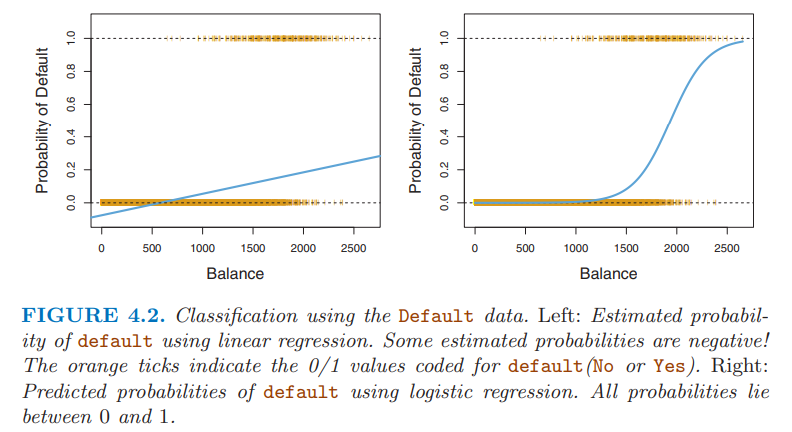
\includegraphics[scale=0.8]{images/logistic_reg.png}
\end{center}
The values of $P(default = Yes|balance)$, which we abbreviate $p(balance)$, will range between 0 and 1. One might predict $default = Yes$ for any individual for whom $p(balance) > 0.5$.\\\\
How should we model the relationship between $p(X) = P(Y = 1|X)$ and $X$? In section \ref{lin_reg} we talked of using a linear regression model to represent
these probabilities:
\[p(X) = \beta_0 + \beta_1X\]
If we use this approach to predict $default=Yes$ using $balance$, for balances close to zero we predict a negative probability of default. To avoid this problem, we must model $p(X)$ using a function that gives outputs between 0 and 1 for all values of $X$. Many functions meet this description. In logistic regression, we use the \textit{logistic function}:
\begin{equation}
    p(X) = \frac{e^{\beta_0 + \beta_1X}}{1 + e^{\beta_0 + \beta_1X}}
    \label{log_reg}
\end{equation}
To fit the model \ref{log_reg}, we use a method called maximum likelihood, which we discuss in the next section. The logistic function will always produce
an \textit{S-shaped} curve, and so regardless of the value of $X$, we will obtain a sensible prediction. After a bit of manipulation of \ref{log_reg}, we find that
\begin{equation}
    \frac{p(X)}{1 - p(X)} = e^{\beta_0 + \beta_1X}
    \label{odds}
\end{equation}
The quantity $p(X)/[1-p(X)]$ is called \textit{the odds}. Values of the odds close to 0 and $\infty$ indicate very low and very high probabilities of default, respectively. For example, on average 1 in 5 people with an odds of 1/4 will default, since p$(X)=0.2$ implies an odds of $\frac{0.2}{1 - 0.2} = 1/4$. By taking the logarithm of both sides of $\ref{odds}$, we arrive at:
\[log\left(\frac{p(X)}{1 - p(X)}\right) = \beta_0 + \beta_1X\]
The left-hand side is called the \textit{log-odds} or \textit{logit}. In a linear regression model, $\beta_1$ gives the average change in $Y$ associated with a one-unit increase in $X$. In contrast, in a logistic regression model, increasing $X$ by one unit changes the log odds by $\beta_1$. However, because the relationship between $p(X)$ and $X$ in \ref{log_reg} is not a straight line, $\beta_1$ does not correspond to the change in $p(X)$ associated with a one-unit increase in $X$. The amount that $p(X)$ changes due to a one-unit change in $X$ will depend on the current value of $X$. But regardless of the value of $X$, if $\beta_1$ is positive then increasing $X$ will be associated with increasing $p(X)$, and if $\beta_1$ is negative then increasing $X$ will be associated with decreasing $p(X)$.

\subsection{Estimating the Regression Coefficients}
The coefficients $\beta_0$ and $\beta_1$ in \ref{log_reg} are unknown, and must be estimated based on the available training data. Although we could use (non-linear) least squares, the more general method of maximum likelihood is preferred, since it has better statistical properties. The basic intuition behind using maximum likelihood
to fit a logistic regression model is as follows: we seek estimates for $\beta_0$ and
$\beta_1$ such that the predicted probability $\hat{p}(xi)$ of default for each individual, using \ref{log_reg}, corresponds as closely as possible to the individual’s observed default status. This intuition can be formalized using a mathematical equation called a \textit{likelihood function}:
\[l(\beta_0, \beta_1) = \prod_{i:y_i = 1} p(x_i) \prod_{i':y_{i'}=0} (1 - p(x_{i'}))\]
The estimates $\hat\beta_0$ and $\hat\beta_1$ are chosen to \textit{maximize} this likelihood function. In the linear regression setting, the least squares approach is in fact a special case of maximum likelihood. Once the coefficients have been estimated, it is a simple matter to compute the probability by plugging  $\hat\beta_0$ and $\hat\beta_1$ into \ref{log_reg}.

\subsection{Multiple Logistic Regression}
We now consider the problem of predicting a binary response using multiple predictors. By analogy with the extension from simple to multiple linear regression, we can generalize as follows:
\[log\left(\frac{p(X)}{1 - p(X)}\right) = \beta_0 + \beta_1 X_1 + ... + \beta_p X_p\]
Just as before, we use the maximum likelihood method to estimate the coefficients.

\subsection{Logistic Regression for $>2$ Response Classes}
We sometimes wish to classify a response variable that has more than two classes. The two-class logistic regression models discussed in the previous sections have multiple-class extensions, but in practice they tend not to be used all that often. One of the reasons is that the method we discuss in the next section, \textit{discriminant analysis}, is popular for multiple-class classification. So we do not go into the details of multiple-class logistic regression here.

\section{Linear Discriminant Analysis}
Logistic regression involves directly modeling $Pr(Y = k|X = x)$ using the logistic function. We now consider an alternative and less direct approach to estimating these probabilities. In this alternative approach, we model the distribution of the predictors $X$ separately in each of the response classes (i.e. given $Y$), and then use Bayes’ theorem to flip these around into estimates for $Pr(Y = k|X = x)$. Why do we need another method, when we have logistic regression? There are several reasons:
\begin{itemize}
    \item When the classes are well-separated, the parameter estimates for the logistic regression model are surprisingly unstable. Linear discriminant analysis does not suffer from this problem.

    \item If $n$ is small and the distribution of the predictors X is approximately normal in each of the classes, the linear discriminant model is again more stable than the logistic regression model.

    \item Linear discriminant analysis is popular when we have more than two response classes.
\end{itemize}

\subsection{Using Bayes’ Theorem for Classification}
Suppose that we wish to classify an observation into one of $K$ classes, where $K > 2$. Let $\pi_k$ represent the overall or prior probability that a randomly chosen observation comes from the $k$th class; Let $f_k(X) \equiv Pr(X = x|Y = k)$ denote the density function of $X$ for an observation that comes from the $k$th class. In other words, $f_k(x)$ is relatively large if there is a high probability that an observation in the $k$th class has $X \approx x$, and it is small otherwise. Then Bayes’
theorem states that \footnote{Note that the denominator serves to normalize the probability between 0 and 1}:
\begin{equation}
    Pr(Y = k|X = x) = \frac{\pi_k f_k(x)}{\sum_{l=1}^K \pi_l f_l(x)}
    \label{lda}
\end{equation}
In accordance with our earlier notation, we will use the abbreviation $p_k(X)
= Pr(Y = k|X)$. Then, we just need to estimate $\pi_k$ and $f_k(X)$ and plug them into \ref{lda} to make a prediction. In general, estimating $\pi_k$ is easy,  we simply compute the fraction of the training observations that belong to the $k$th class. However, estimating $f_k(X)$ tends to be more challenging, unless we assume some simple forms for these densities.\\\\
We know that the Bayes classifier, which classifies an observation to the class for which $p_k(X)$ is largest, has the lowest possible error rate out of all classifiers. If we can find a way to estimate $f_k(X)$, then we can develop a classifier that approximates the Bayes classifier.

\subsection{Linear Discriminant Analysis for $p = 1$}
For now, assume that p = 1, that is, we have only one predictor. We would like to obtain an estimate for $f_k(x)$ that we can plug into \ref{lda}. We will then classify an observation to the class for which $p_k(x)$ is greatest.\\\\
Suppose we assume that $f_k(x)$ is normal or Gaussian. In the one-dimensional setting, the normal density takes the form
\begin{equation}
    f_k(x) = \frac{1}{\sqrt{2\pi}\sigma_k}\text{exp}\left(-\frac{1}{2\sigma_k^2}(x - \mu_k)^2  \right)
    \label{normal_distr}
\end{equation}
where $\mu_k$ and $\sigma_k^2$ are the mean and variance parameters for the $k$th class. For now, let us further assume that $\sigma_1^2 = ... = \sigma_K^2$: that is, there is a shared variance term across all $K$ classes, which for simplicity we can denote by $\sigma^2$. Plugging \ref{normal_distr} into \ref{lda}, we find that
\begin{equation}
    p_k(x) = \frac{\pi_k \frac{1}{\sqrt{2\pi}\sigma}\text{exp}(-\frac{1}{2\sigma^2}(x - \mu_k)^2)}{\sum_{l=1}^K \pi_l \frac{1}{\sqrt{2\pi}\sigma}\text{exp}(-\frac{1}{2\sigma^2}(x - \mu_l)^2)}
    \label{lda_2}
\end{equation}
The Bayes classifier involves assigning an observation X = x to the class for which \ref{lda_2} is largest. Taking the log of \ref{lda_2} and rearranging the terms, it is not hard to show that this is equivalent to assigning the observation to the class for which
\begin{equation}
    \delta_k(x) = x \cdot \frac{\mu_k}{\sigma^2} - \frac{\mu_k^2}{2\sigma^2} + \text{log}(\pi_k)
    \label{discriminant}
\end{equation}
is largest.
\\\\
In practice, even if we are quite certain of our assumption that $X$ is drawn from a Gaussian distribution within each class, we still have to estimate the parameters $\mu_1,...,\mu_K, \pi_1,...,\pi_K$, and $\sigma^2$. The \textit{linear discriminant analysis} (LDA) method approximates the Bayes classifier by computing the following estimates
\[\begin{split}
    \hat{\mu}_k & = \frac{1}{n_k}\sum_{i:y_i = k}x_i\\
    \hat{\sigma}^2 & = \frac{1}{n - K}\sum_{k=1}^K\sum_{i:y_i = k} (x_i - \hat{\mu}_k)^2
\end{split}\] 
where $n$ is the total number of training observations, and $n_k$ is the number of training observations in the $k$th class. The estimate for $\mu_k$ is simply the average of all the training observations from the $k$th class, while $\hat{\sigma}^2$ can be seen as a weighted average of the sample variances for each of the $K$ classes. The LDA classifier plugs these estimates in \ref{discriminant} to make a prediction. The word linear in the classifier’s name stems from the fact that the \textit{discriminant functions} $\delta_k(x)$  are linear functions of $x$.

\subsection{Linear Discriminant Analysis for $p >1$}
We now extend the LDA classifier to the case of multiple predictors. To
do this, we will assume that $X = (X_1, X_2,...,X_p)$ is drawn from a multivariate Gaussian distribution with a class-specific mean vector and a common covariance matrix. The multivariate Gaussian distribution assumes that each individual predictor follows a one-dimensional normal distribution  with some correlation between each pair of predictors.\\\\
To indicate that a $p$-dimensional random variable $X$ has a multivariate Gaussian distribution, we write $X \sim N(\mu, \Sigma)$. Here $E(X) = \mu$ is the mean of $X$ (a vector with p components), and $Cov(X) = \Sigma$ is the $p \times p$ covariance matrix of $X$. 
In the case of $p > 1$ predictors, the LDA classifier assumes that the
observations in the $k$th class are drawn from a multivariate Gaussian distribution $N(\mu_k, \Sigma)$, where $\mu_k$ is a class-specific mean vector, and $\Sigma$ is a covariance matrix that is common to all $K$ classes. In particular $\mu_k$ is a $k$-dimensional vector with one value per class, while $\Sigma$ is a matrix which contains covariances between predictors.
\\\\
The density function $f_k(x)$, the discriminant function $\delta_k(x)$ and the subsequent prediction process are generalization of the ones presented before. Also the estimate of the parameters is done in a similar way as in the one-dimensional case.\\\\
We can perform LDA on the \textbf{Default} data in order to predict whether
or not an individual will default on the basis of credit card balance and student status. The LDA model fit to the 10, 000 training samples results
in a training error rate of 2.75\%. This sounds like a low error rate, but two caveats must be noted.
\begin{itemize}
    \item First of all, training error rates will usually be lower than test error rates, which are the real quantity of interest. The higher the ratio of parameters $p$ to number of samples $n$, the more we expect this overfitting to play a role.

    \item Second, since only 3.33\% of the individuals in the training sample defaulted, a simple but useless classifier that always predicts that each individual will not default, regardless of his or her credit card balance and student status, will result in an error rate of 3.33\%. In other words, the trivial null classifier will achieve an error rate that is only a bit higher than the LDA training set error rate.
\end{itemize}
In practice, a binary classifier such as this one can make two types of
errors: it can incorrectly assign an individual who defaults to the no default category, or it can incorrectly assign an individual who does not default to the default category. It is often of interest to determine which of these two types of errors are being made.
\begin{center}
    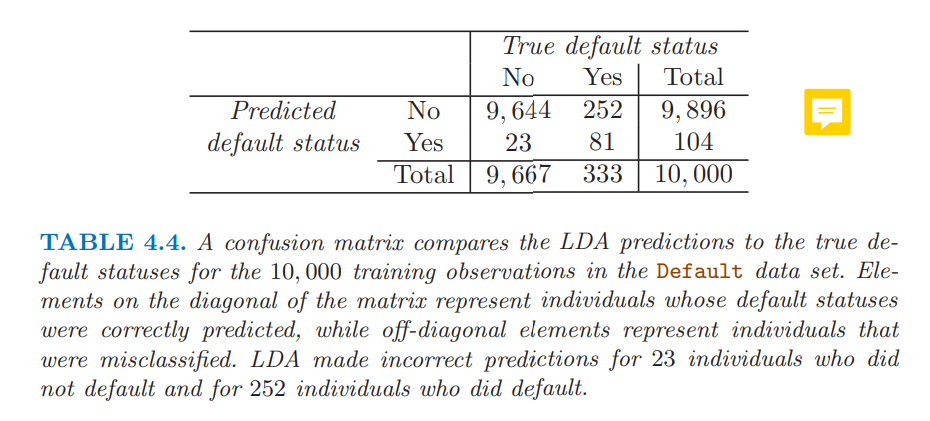
\includegraphics[scale=0.8]{images/confusion-matrix.png}
\end{center}
A \textit{confusion matrix}, shown in the Table above, is a convenient way to display this information. The table reveals that LDA predicted that a total of 104 people would default. Of these people, 81 actually defaulted and 23 did not. Hence only 23 out of 9, 667 of the individuals who did not default were incorrectly labeled. This looks like a pretty low error rate! However, of the 333 individuals who defaulted, 252 (or 75.7\%) were missed by LDA. So while the overall error rate is low, the error rate among individuals who defaulted is very high.\\\\
Class-specific performance is also important in medicine and biology,
where the terms \textit{sensitivity} and \textit{specificity} characterize the performance of a classifier or screening test. In this case the sensitivity is the percentage of true defaulters that are identified, a low 24.3\% in this case. The specificity is the percentage of non-defaulters that are correctly identified, here 9644/9667 = 99,8\%. More in general, the sensitivity is given by $TP/(TP + FN)$, where $TP$ and $FN$ stand for True Positive and False Negative, while the specificity is given by $TN/(TN + FP)$, where $TN$ and $FP$ stand for True Negative and False Positive. The accuracy is instead given by $(TP + TN) / Total = (9644 + 81) / 10000 = 97,25\%$. From the perspective of a credit card company that is trying to identify high-risk individuals, minimize the number of false negative is crucial.\\\\
Why does LDA do such a poor job of classifying the customers who default? As we have
seen, LDA is trying to approximate the Bayes classifier, which has the lowest total error rate out of all classifiers (if the Gaussian model is correct). That is, the Bayes classifier will yield the smallest possible total number of misclassified observations, irrespective of which class the errors come from. We will now see that it is possible to modify LDA in order to develop a classifier that better meets the credit card company’s needs.\\\\
The Bayes classifier works by assigning an observation to the class for which the posterior probability $p_k(X)$ is greatest. In the two-class case, the Bayes classifier, and by extension LDA, uses a threshold of 50\% for the posterior probability of default in order to assign an observation to the default class. However, if we are concerned about incorrectly predicting the default status for individuals who default, then we can consider
lowering this threshold. For instance, we might label any customer with a
posterior probability of default above 20\% to the default class.
\[Pr(default = Yes|X = x) > 0.2\]
With this modification, the classifier will have less false negative, but more false positive.\\\\
How can we decide which threshold value is best? Such a decision must be based on domain knowledge, such as detailed information about the costs associated with default. The \textit{ROC curve} is a popular graphic for simultaneously displaying the two types of errors for all possible thresholds. The overall performance of a classifier, summarized over all possible thresholds, is given by the area under the (ROC) curve (AUC). An ideal ROC curve will hug the top left corner, so the larger the AUC the better the classifier.
\begin{center}
    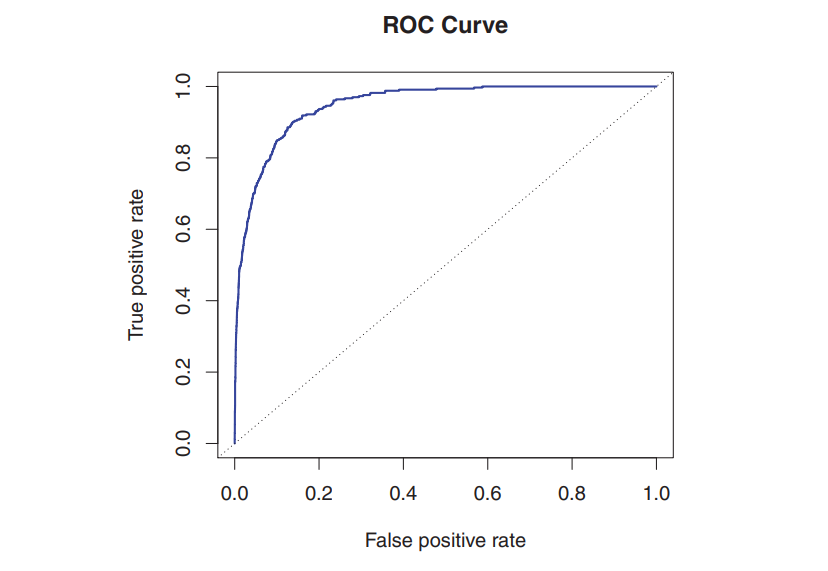
\includegraphics[scale=0.7]{images/ROC.png}
\end{center}
The Figure above shows A ROC curve for the LDA classifier on the Default data. It traces out two types of error as we vary the threshold value for the posterior probability of default. The actual thresholds are not shown. The true positive rate
is the sensitivity. The false positive rate is 1-specificity  The ideal ROC curve hugs the top left corner, indicating a high true positive rate and a low false positive rate. The dotted line represents the random classifier. The best threshold is the one associated with the value closest to the top-left corner. For more information about ROC curve visit the following post: \href{https://towardsdatascience.com/understanding-auc-roc-curve-68b2303cc9c5}{ROC CURVE}.

\section{Quadratic Discriminant Analysis}
As we have discussed, LDA assumes that the observations within each class are drawn from a multivariate Gaussian distribution with a class specific mean vector and a covariance matrix that is common to all K classes. Quadratic discriminant analysis (QDA) provides an alternative approach. Like LDA, the QDA classifier results from assuming that the observations from each class are drawn from a Gaussian distribution, and plugging estimates for the parameters into Bayes’ theorem in order to perform prediction. However, unlike LDA, QDA assumes that each class has its own covariance matrix. Unlike LDA, the quantity $x$ appears as a quadratic function in the discriminant function of QDA.\\\\
Why would one prefer LDA to QDA, or vice-versa? The answer lies in the bias-variance trade-off. When there are $p$ predictors, then estimating a covariance matrix requires estimating $p(p+1)/2$ parameters. QDA estimates a separate covariance matrix for each class, for a total of $Kp(p+1)/2$ parameters.  LDA is a much less flexible classifier than QDA, and so has substantially lower variance. This can potentially lead to improved prediction performance. But there is a trade-off: if LDA’s assumption that the $K$ classes share a common covariance matrix is badly off, then LDA can suffer from high bias. LDA tends to be a better bet than QDA if there are relatively few training observations and so reducing variance is crucial. In contrast, QDA is recommended if the training set is very large, so that the variance of the classifier is not a major concern, or if the assumption of a common covariance matrix for the $K$ classes is clearly untenable.

\section{A Comparison of Classification Methods}
Though their motivations differ, the logistic regression and LDA methods are closely connected. Both logistic regression and LDA produce linear decision boundaries. The only difference between the two approaches lies in how they estimate the parameters, logistic regression uses maximum likelihood, while LDA uses the estimated mean and variance from a normal distribution.
\\\\
LDA assumes that the observations are drawn from a Gaussian distribution with a common covariance matrix in each class, and so can provide some improvements over logistic regression when this assumption approximately holds. Conversely, logistic regression can outperform LDA if these Gaussian assumptions are not met.\\\\
KNN takes a completely different approach from the classifiers seen in this chapter. It is a completely non-parametric approach: no assumptions are made about the shape of the decision boundary. Therefore, we can expect this approach to dominate LDA and logistic regression when the decision boundary is highly non-linear. On the other hand, KNN does not tell us which predictors are important.\\\\
Finally, QDA serves as a compromise between the non-parametric KNN method and the linear LDA and logistic regression approaches. Since QDA assumes a quadratic decision boundary, it can accurately model a wider range of problems than can the linear methods.
